\documentclass[12pt, twoside]{article}
\usepackage[letterpaper, margin=1in, headsep=0.5in]{geometry}
\usepackage[english]{babel}
\usepackage[utf8]{inputenc}
\usepackage{amsmath}
\usepackage{amsfonts}
\usepackage{amssymb}
\usepackage{tikz}
\usepackage{yhmath}
%\usetikzlibrary{quotes, angles}

\usepackage{graphicx}
\usepackage{enumitem}
\usepackage{multicol}

\usepackage{fancyhdr}
\pagestyle{fancy}
\fancyhf{}
\renewcommand{\headrulewidth}{0pt} % disable the underline of the header

\fancyhead[RE]{\thepage}
\fancyhead[RO]{\thepage \\ Name: \hspace{3cm}}
\fancyhead[L]{BECA / Dr. Huson / 10th Grade Geometry\\* 29 January 2020}

\begin{document}
\subsubsection*{8.2b Do Now: Estimating and measuring angles, length, and area}
 \begin{enumerate}

  \item In your notebook, write the formulas for the area and circumference of circles:
\[A=\pi r^2\]
\[C=\pi D = 2\pi r\]

  \item Given the circle centered at $O$ with radius $r=5$.
  \begin{multicols}{2}
    \begin{enumerate}
      \item Find the circumference of a circle. %\vspace{1cm}
      \item Find the area of the circle.\vspace{3cm}
    \end{enumerate}
    %\columnbreak
    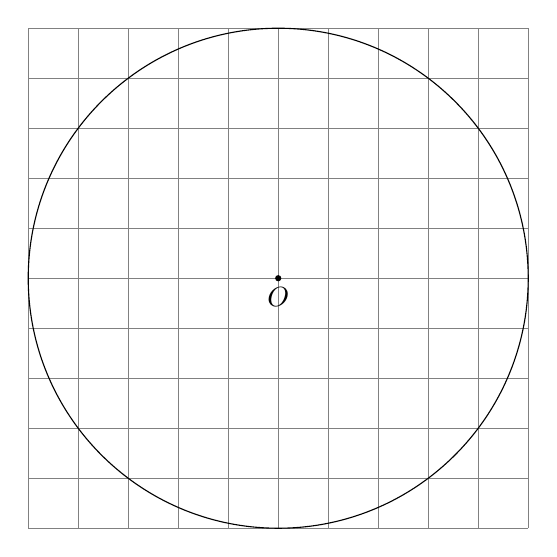
\begin{tikzpicture}[scale=.635]
      \draw [help lines] (-5,-5) grid (5,5);
      %\draw [thick, ->] (-2.2,0) -- (10.4,0) node [below right] {$x$};
      %\draw [thick, ->] (0,-2.2)--(0,10.4) node [left] {$y$};
      \draw (0,0) circle [radius=5] node[below]{$O$};
      \draw [fill] (0,0) circle [radius=0.05];
    \end{tikzpicture}
  \end{multicols}

  \item Given the semi-circle shown with diameter $AB=8$. Find its area and perimeter.
    \begin{flushright}
    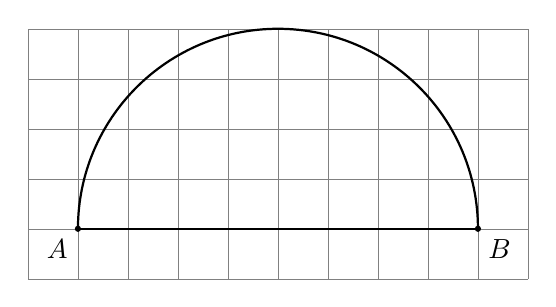
\begin{tikzpicture}[scale=.635]
      \draw [help lines] (-5,-1) grid (5,4);
      \draw [thick] (-4,0)node[below left]{$A$} -- (4,0)node[below right]{$B$};
      %\draw [thick, ->] (0,-2.2)--(0,10.4) node [left] {$y$};
      \draw [thick] (4,0) arc (0:180:4);
      \draw [fill] (-4,0) circle [radius=0.05];
      \draw [fill] (4,0) circle [radius=0.05];
    \end{tikzpicture}
  \end{flushright} \vspace{1cm}

  \item Find the radius of a circle having an area of $49 \pi$. \vspace{2cm}
  \item Find the diameter of a circle with a circumference of 62.832.

\newpage 
\subsubsection*{Classwork: Estimating and measuring angles, length, and area} 
  \item Find the area of a semi-circle with radius of 7 centimeters. \vspace{2cm}

  \item Given circle $O$ with radius $OB=3$ cm.
    \begin{multicols}{2}
    \raggedcolumns
    \begin{enumerate}
      \item Find the circumference of circle $O$. \vspace{1.7cm}
      \item Find the area of the circle.  \vspace{2cm}
      \item A hexagon is inscribed in the circle, with $A$ and $B$ two of its vertices. \\[0.25cm]
      Find the area of the sector $AOB$. \vspace{1.5cm}
    \end{enumerate}
      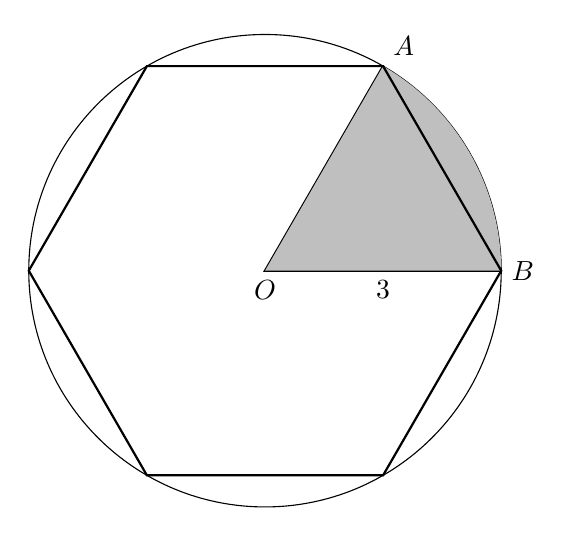
\begin{tikzpicture}[scale=1]
        \draw (0,0) circle[radius=3];
        \draw [thick]
        (0:3) node[right] {$B$}--
        (0,0) node[below] {$O$}--
        (60:3) node[above right] {$A$};
        \fill [lightgray]
        (0,0)--(0:3) arc (0:60:3)--(0,0);
        \draw (1.5,0) node[below] {$3$};
        \draw [thick] (0:3)--(60:3)--(120:3)--(180:3)--
        (240:3)--(300:3)--cycle;
      \end{tikzpicture}
    \end{multicols}  \vspace{4cm}

  \item Find the volume of a pyramid ($V=\frac{1}{3}Bh$) having a height of 11.3 inches and with a square base having side lengths of 7 inches. Express your result to the \emph{nearest cubic inch}. \vspace{5cm}

\newpage
  \item Find the volume of a hemisphere with a radius of 30 inches, to the \emph{nearest whole cubic inch}. (The formula for the volume of a \emph{sphere} is $V=\frac{4}{3}\pi r^3$) \vspace{5cm}

  \item Given $R(-2,0)$ and $S(3,5)$, find the length of $\overline{RS}$. Simplify the radical. \vspace{4cm}

  \item On the graph, draw polygon ABCDEF with vertices A(1, 1), B(1, 4), C(3, 4), D(3, 7), E(8, 7), and F(8, 1). Find the perimeter and the area of the polygon.\\[1cm]
  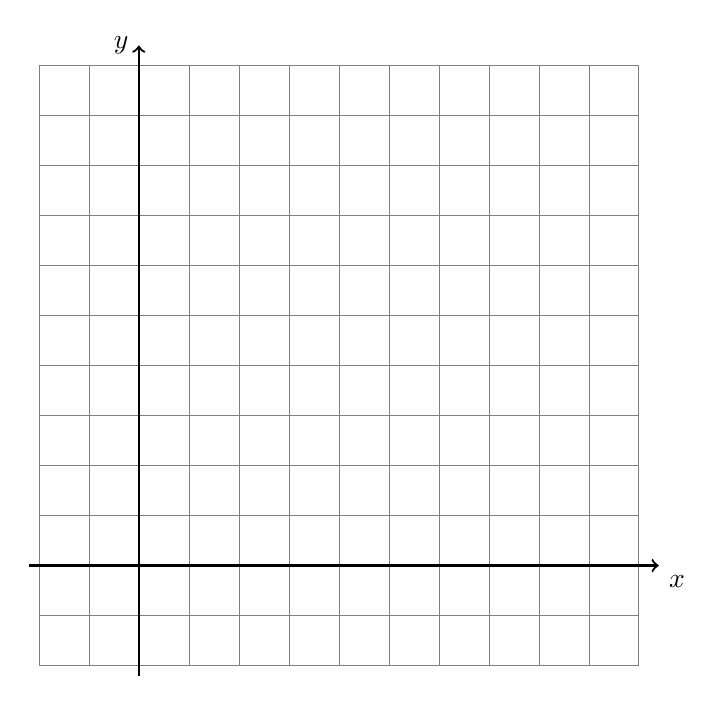
\begin{tikzpicture}[scale=.635]
    \draw [help lines] (-2,-2) grid (10,10);
    \draw [thick, ->] (-2.2,0) -- (10.4,0) node [below right] {$x$};
    \draw [thick, ->] (0,-2.2)--(0,10.4) node [left] {$y$};
  \end{tikzpicture}
  \vspace{2cm}

\newpage
\subsubsection*{Estimating and measuring}
  \item The point $P$ falls $A(0)$ and $B(10)$ on the numberline $\overleftrightarrow{AB}$ as shown below. \\[15pt] % Midpoint
  \begin{tikzpicture}
    \draw [<->] (-0.5,0)--(10.5,0);
    \foreach \x in {0,10} %2 leading for diff!=1
      \draw[shift={(\x,0)},color=black] (0pt,-3pt) -- (0pt,3pt) node[below=5pt]  {$\x$};
      \draw [fill] (0,0) circle [radius=0.05] node[above] {$A$};
      \draw [fill] (10,0) circle [radius=0.05] node[above] {$B$};
      \draw [fill] (2*3.1416,0) circle [radius=0.05] node[above] {$P$};
  \end{tikzpicture}
  \begin{enumerate}
    \item Estimate the value of $P$ without using any tools. \vspace{1cm} 
    \item Find the position of $P$ as accurately as you can with a ruler. 
  \end{enumerate} \vspace{1cm} 

  \item The distance from $B$ on the line is scaled so that each centimeter represents one foot. \\[15pt] % Midpoint
  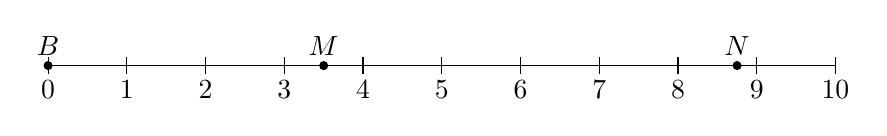
\begin{tikzpicture}
    \draw [-] (0,0)--(10,0);
    \foreach \x in {0,...,10} %2 leading for diff!=1
      \draw[shift={(\x,0)},color=black] (0pt,-3pt) -- (0pt,3pt) node[below=5pt]  {$\x$};
      \draw [fill] (0,0) circle [radius=0.05] node[above] {$B$};
      \draw [fill] (3.5,0) circle [radius=0.05] node[above] {$M$};
      \draw [fill] (8.75,0) circle [radius=0.05] node[above] {$N$};
  \end{tikzpicture}
  \begin{enumerate}
    \item Estimate the distance of $M$ from $B$ in feet and inches (by eye). \vspace{1cm} 
    \item Using a ruler, find the distance between $M$ and $N$ in feet and inches. 
  \end{enumerate} \vspace{2cm}

  \item Given the circle $O$ with diameter $D=4$.
  \begin{multicols}{2}
    \begin{enumerate}[itemsep=1.5cm]
      \item Estimate the area by counting the squares in the grid.
      \item Calculate the area. 
      \item Quantify the error in your estimate as a percentage.
    \end{enumerate}
    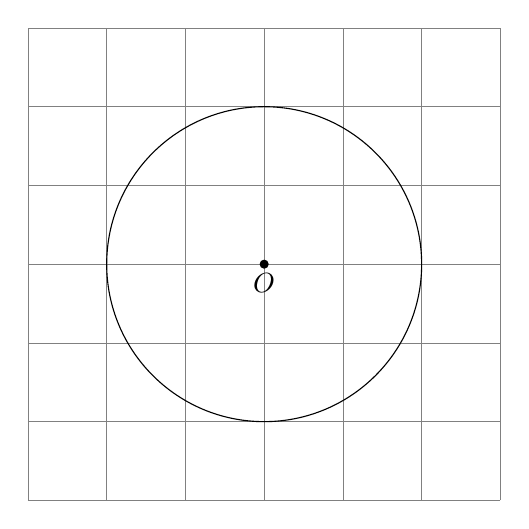
\begin{tikzpicture}[scale=1]
      \draw [help lines] (-3,-3) grid (3,3);
      %\draw [thick, ->] (-2.2,0) -- (10.4,0) node [below right] {$x$};
      %\draw [thick, ->] (0,-2.2)--(0,10.4) node [left] {$y$};
      \draw (0,0) circle [radius=2] node[below]{$O$};
      \draw [fill] (0,0) circle [radius=0.05];
    \end{tikzpicture}
  \end{multicols}


\newpage
  \item Given circle $O$ with chords $\overline{AD}$ and $\overline{BE}$ intersecting at $C$, as shown in the diagram. Use a protractor to measure each angle.
    \begin{multicols}{2}
    \raggedcolumns
    \begin{enumerate}[itemsep=1cm]
      \item Find the $m\angle A$.
      \item Find the $m\angle B$.
      \item Find the $m\angle D$.
      \item Find the $m\angle E$.
      
      \item Given that $BE=8$ \\[0.25cm] 
      Find $BC$.
      \item Find $EC$.
    \end{enumerate}
    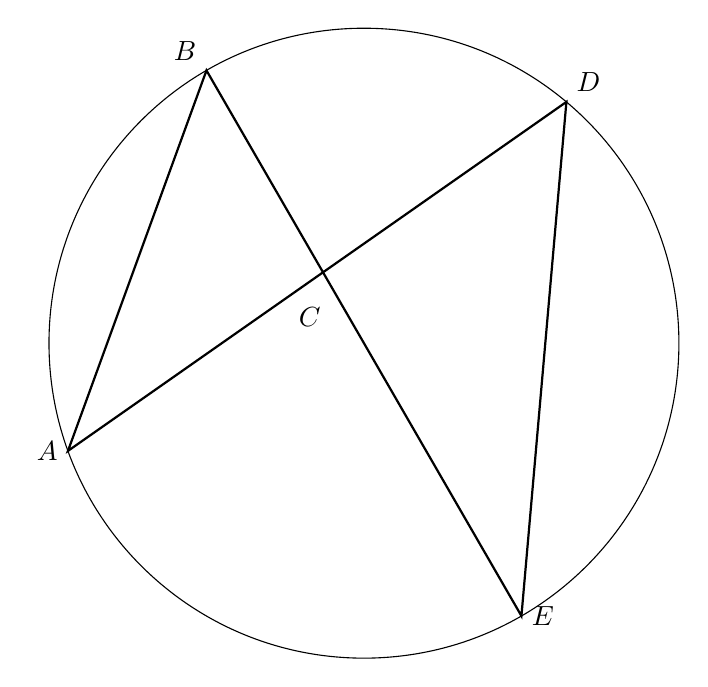
\begin{tikzpicture}[scale=1]
      \draw (0,0) circle[radius=4];
      \draw [thick]
      (-60:4) node[right] {$E$}--
      (120:4) node[above left] {$B$}--
      (200:4) node[left] {$A$}--
      (50:4) node[above right] {$D$}--cycle;
      \draw (140:0.9) node[below] {$C$};
    \end{tikzpicture}
    \end{multicols}
  \vspace{2cm}

  \item The diagram below is drawn to scale. Given that $BE=10$ and $DE=5$, find $AC$.
  \begin{center}
    \begin{tikzpicture}[scale=1]
      \coordinate [label=left:$A$](A) at (-12,6);
      \coordinate [label=below:$B$](B) at (0, 0);
      \coordinate [label=below left:$C$](C) at (-12,0);
      \coordinate [label=above:$D$](D) at (-8, 4);
      \coordinate [label=below:$E$](E) at (-8,0);
      \draw [thick] (A)--(B)--(C)--cycle;
      \draw [thick] (A)--(C);
      \draw [thick] (D)--(E);
    \end{tikzpicture}
  \end{center}

\end{enumerate}
\end{document}
